Рассмотрим и оценим работу алгоритмов на матрицах $A[M \times N]$ и $B[N \times Q]$. 

\section{Алгоритм Винограда}
\qquadОсновная задача данного алгоритма --- сократить долю умножений в самом тяжёлом, затратном участке кода. Для этого используется формула (\ref{formula3}).\\

Некоторые из слагаемых можно вычислить заранее и использовать повторно для каждой строки первой матрицы и для каждого столбца второй. Таким образом, трудоёмкость алгоритма уменьшается за счёт сокращения количества производимых операций.\\

В этом алгоритме важно учитывать, что при нечётном значении $N$, необходимо вычислять дополнительное слагаемое $u_N \cdot v_N$.\\

\textbf{Схема} алгоритма представлена на Рис.\ref{fig1:image}.\\
\begin{figure}[pt!]
	\begin{center}
		{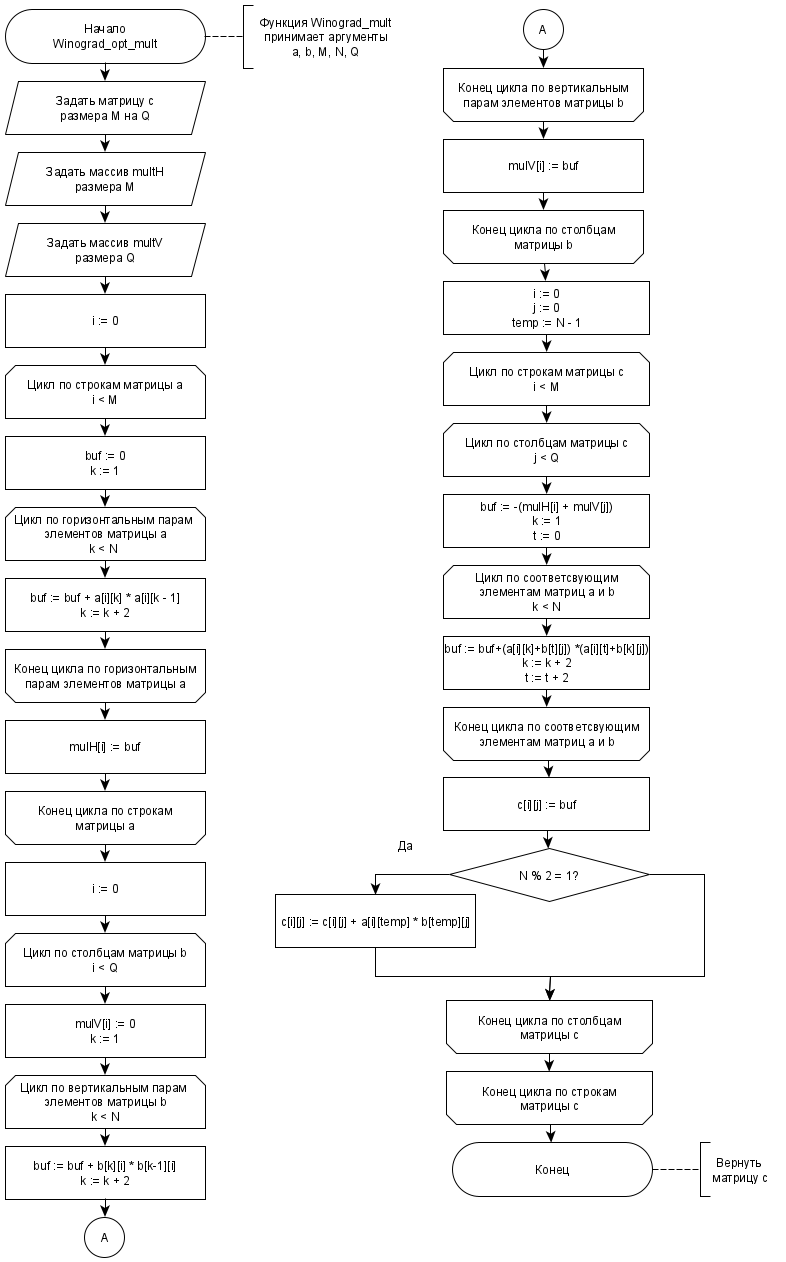
\includegraphics[scale = 0.52]{schemes/opt_winograd}}
		\caption{Алгоритм Винограда}
		\label{fig1:image}
	\end{center}
\end{figure}

\newpage

\section{Распараллеленный алгоритм Винограда (1 вариант)}
\qquadВ этом алгоритме параллельно выполняются вычисления по строкам матрицы $C$. Каждому потоку выделяется строки, начиная с $i$, где $i$ - порядковый номер потока, с шагом $step$ - количество потоков.

\textbf{Схема} алгоритма представлена на Рис.\ref{fig2:image} (главный поток) и на Рис. \ref{fig3:image} (рабочий поток).\\
\begin{figure}[h]
	\begin{center}
		{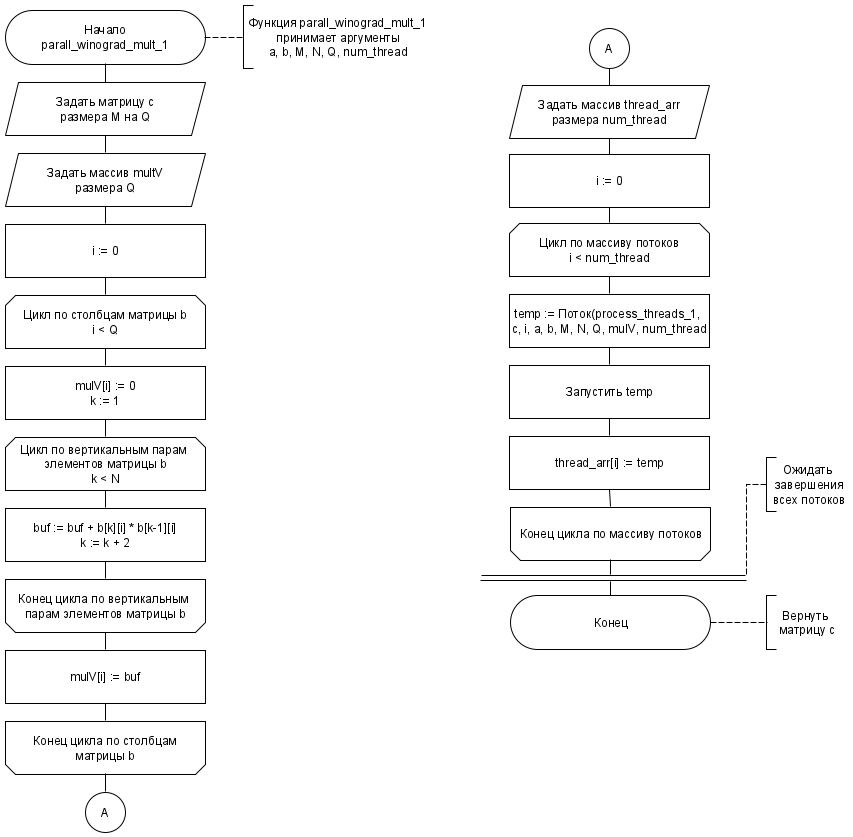
\includegraphics[scale = 0.58]{schemes/parall_1_main}}
		\caption{Распараллеленный алгоритм Винограда (1 вариант). Главный поток}
		\label{fig2:image}
	\end{center}
\end{figure}

\begin{figure}[pt!]
	\begin{center}
		{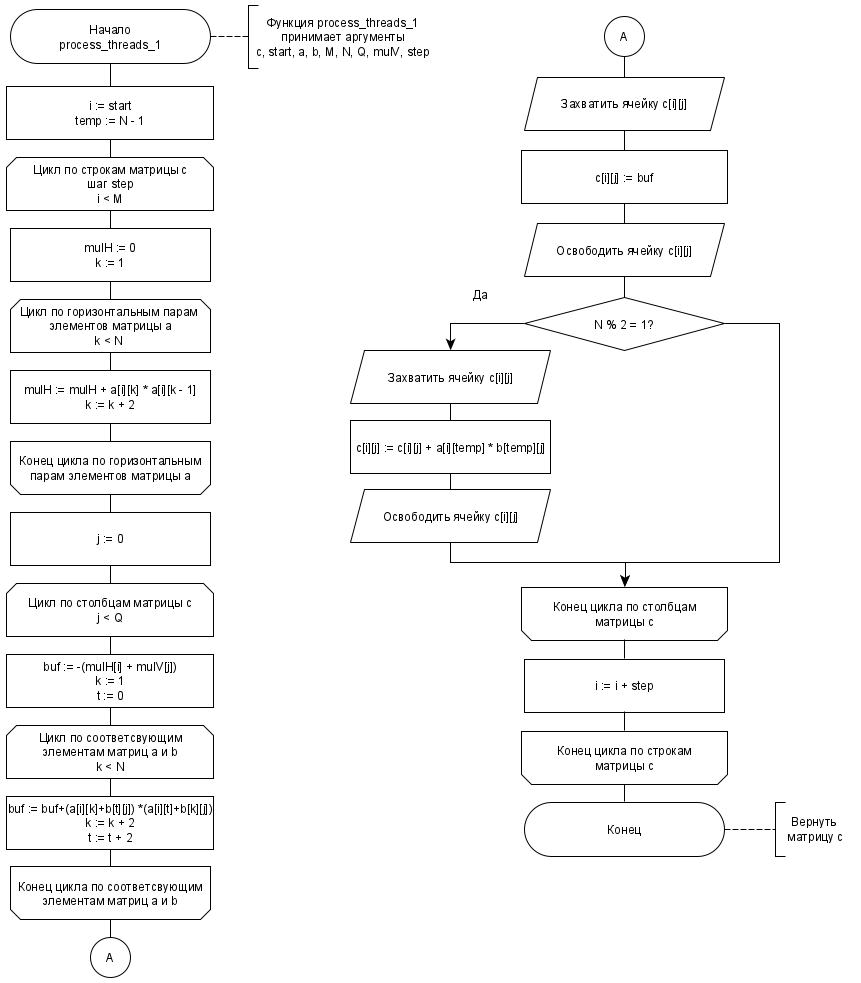
\includegraphics[scale = 0.6]{schemes/parall_1_work}}
		\caption{Распараллеленный алгоритм Винограда (1 вариант). Рабочий поток}
		\label{fig3:image}
	\end{center}
\end{figure}

\newpage

\section{Распараллеленный алгоритм Винограда (2 вариант)}
\qquadВ отличие от предыдущего алгоритма, в этом алгоритме параллельно выполняются вычисления по столбцам. Каждому потоку выделяется столбцы, начиная с $i$, где $i$ - порядковый номер потока, с шагом $step$ - количество потоков.

\textbf{Схема} алгоритма представлена на Рис.\ref{fig4:image} (главный поток) и на Рис. \ref{fig5:image} (рабочий поток).\\
\begin{figure}[h]
	\begin{center}
		{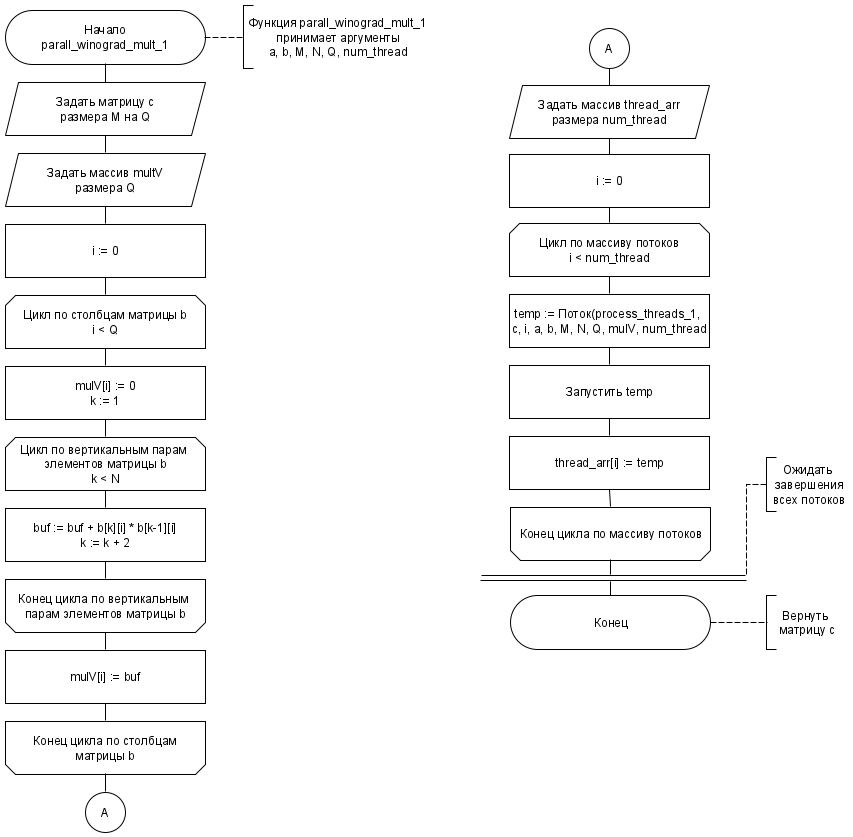
\includegraphics[scale = 0.58]{schemes/parall_1_main}}
		\caption{Распараллеленный алгоритм Винограда (2 вариант). Главный поток}
		\label{fig4:image}
	\end{center}
\end{figure}

\begin{figure}[pt!]
	\begin{center}
		{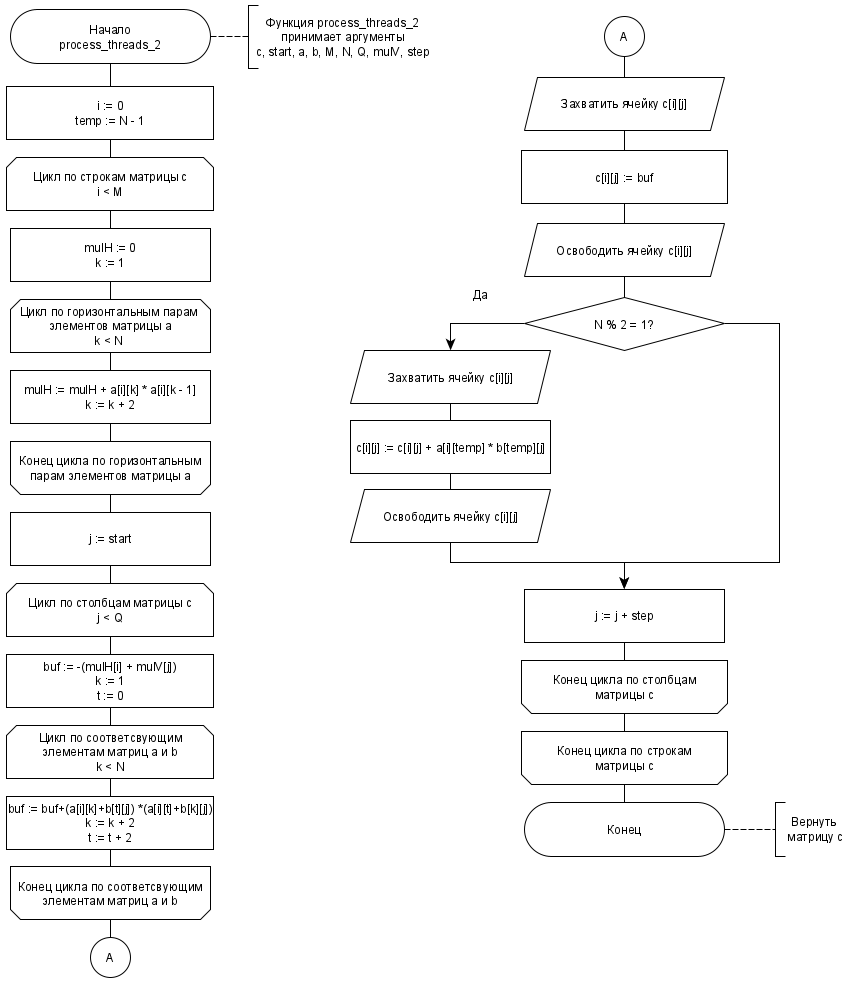
\includegraphics[scale = 0.6]{schemes/parall_2_work}}
		\caption{Распараллеленный алгоритм Винограда (2 вариант). Рабочий поток}
		\label{fig5:image}
	\end{center}
\end{figure}

\section{Требования к ПО}
\qquadДля корректной работы алгоритмов и проведения тестов необходимо выполнить следующее.
\begin{itemize}
	\item Обеспечить возможность ввода двух матриц через консоль.
	\item В случае ввода некорректных данных вывести соответствующее сообщение. Программа не должна аварийно завершаться.
	\item Обеспечить возможность консольного ввода предела количества используемых потоков.
	\item Реализовать функцию замера процессорного времени, которое выбранный метод затрачивает на вычисление результатов. Вывести результаты замеров на экран.
\end{itemize}

\section{Заготовки тестов}
\qquadПри проверке на корректность работы реализованных функций необходимо провести следующие тесты:
\begin{itemize}
	\item один поток;
	\item умножение матриц размером $1 \times 1$;
	\item число потоков меньше, чем $M, N, Q$;
	\item число потоков больше, чем $M, N, Q$.
\end{itemize}

\section*{Вывод}
\addcontentsline{toc}{section}{Вывод}
\qquadВ этом разделе разобраны основные принципы выбранных алгоритмов, построены схемы их работы. Также описаны требования к программному обеспечению и приведены заготовки тестов, которые будут использоваться в дальнейшем.